% Recorded state, input, execution mode and physical poses share elapsed time.
\begin{figure*}[t]
\centering
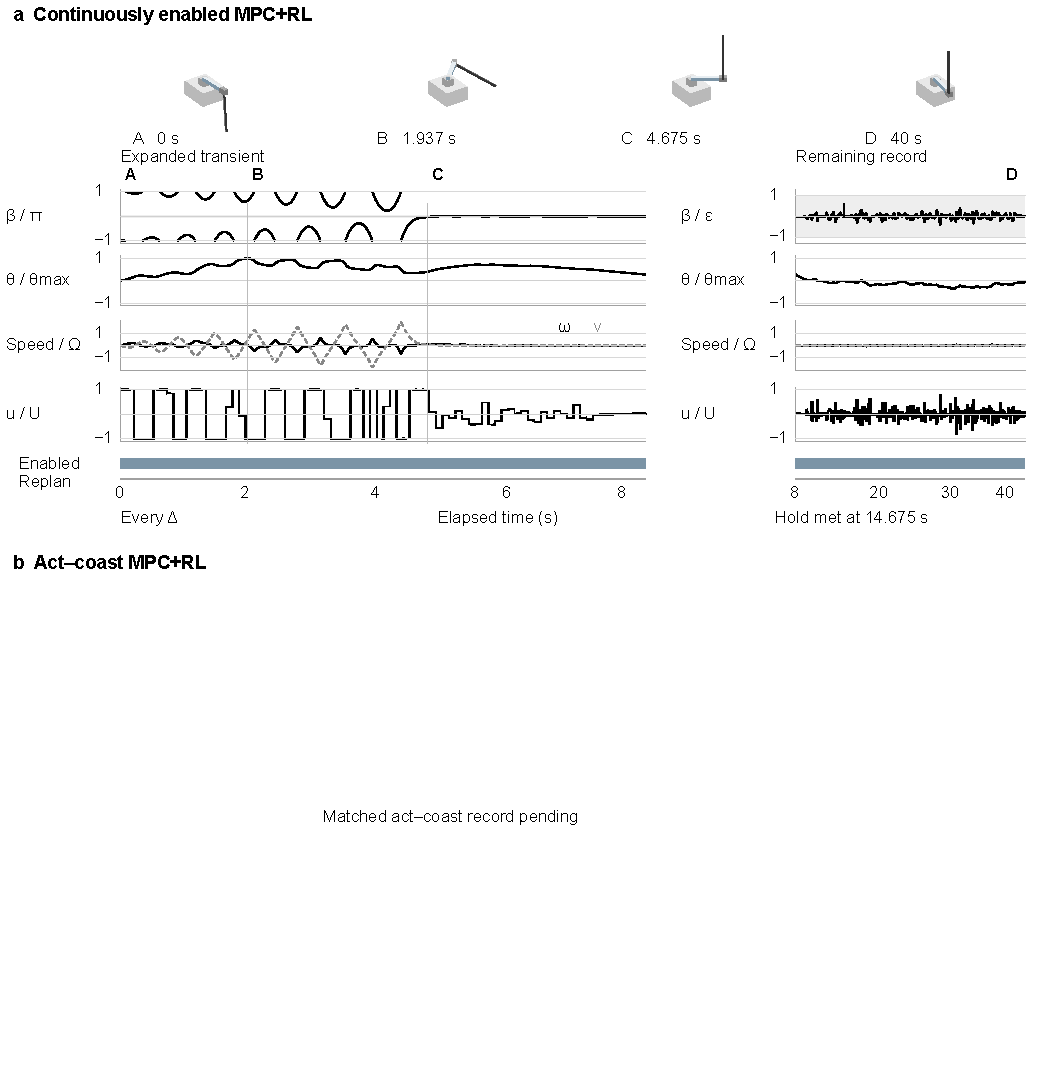
\includegraphics[width=\textwidth]{figures/session-record/figure-4-session-record.pdf}
\caption{Recorded motion and control activity.
(a) The fixed downward-neighborhood MPC+RL session. Adjacent linear views show the expanded initial segment and the complete remainder; no elapsed interval is omitted. Upright error $\beta=\operatorname{wrap}(\alpha-\pi)$ uses $\beta/\pi$ at left and $\beta/\varepsilon$ at right, where $\alpha$ is the pendulum angle from downward, wrapping selects $[-\pi,\pi)$, and $\varepsilon$ is the assessment tolerance. Curve breaks mark angular wrapping, not missing samples. Gray shading denotes this tolerance and the zero line denotes ideal upright orientation. Arm angle $\theta$ is divided by its prescribed bound $\theta_{\max}$; arm speed $\omega$ (black) and pendulum speed $\nu$ (gray dashed) share the downward small-motion frequency $\Omega$. Applied torque $u/U$, with cap $U>0$, is drawn as held commands. The blue rail denotes continuous enablement; torque magnitude does not determine mode. Feedback repeats every command interval $\Delta$. The short tick in the right error plot marks completion of the required holding duration.
Keyframes use one camera and recorded states: A is the initial condition, B the largest arm excursion before first upright-band entry, C that first entry, and D the final state. Their strip is not time-proportional; letters and timestamps identify the matching trace positions.
(b) The matched act--coast record is pending, so its configurations, curves, modes and events remain blank. These are simulated configurations, not hardware observations.}
\label{fig:session-record}
\end{figure*}
